\documentclass{article}

\usepackage{graphicx}
\usepackage{tikz}
\usepackage{tikzsymbols}
\usetikzlibrary{calc,patterns,shapes.geometric}
\pagestyle{empty}
\usepackage[margin=0pt]{geometry}
\geometry{papersize={14in,12in}}

\def\centerarc[#1](#2)(#3:#4:#5){\draw[#1] ($(#2)+({#5*cos(#3)},{#5*sin(#3)})$) arc (#3:#4:#5);}

\begin{document}
	\begin{figure}
		\centering
		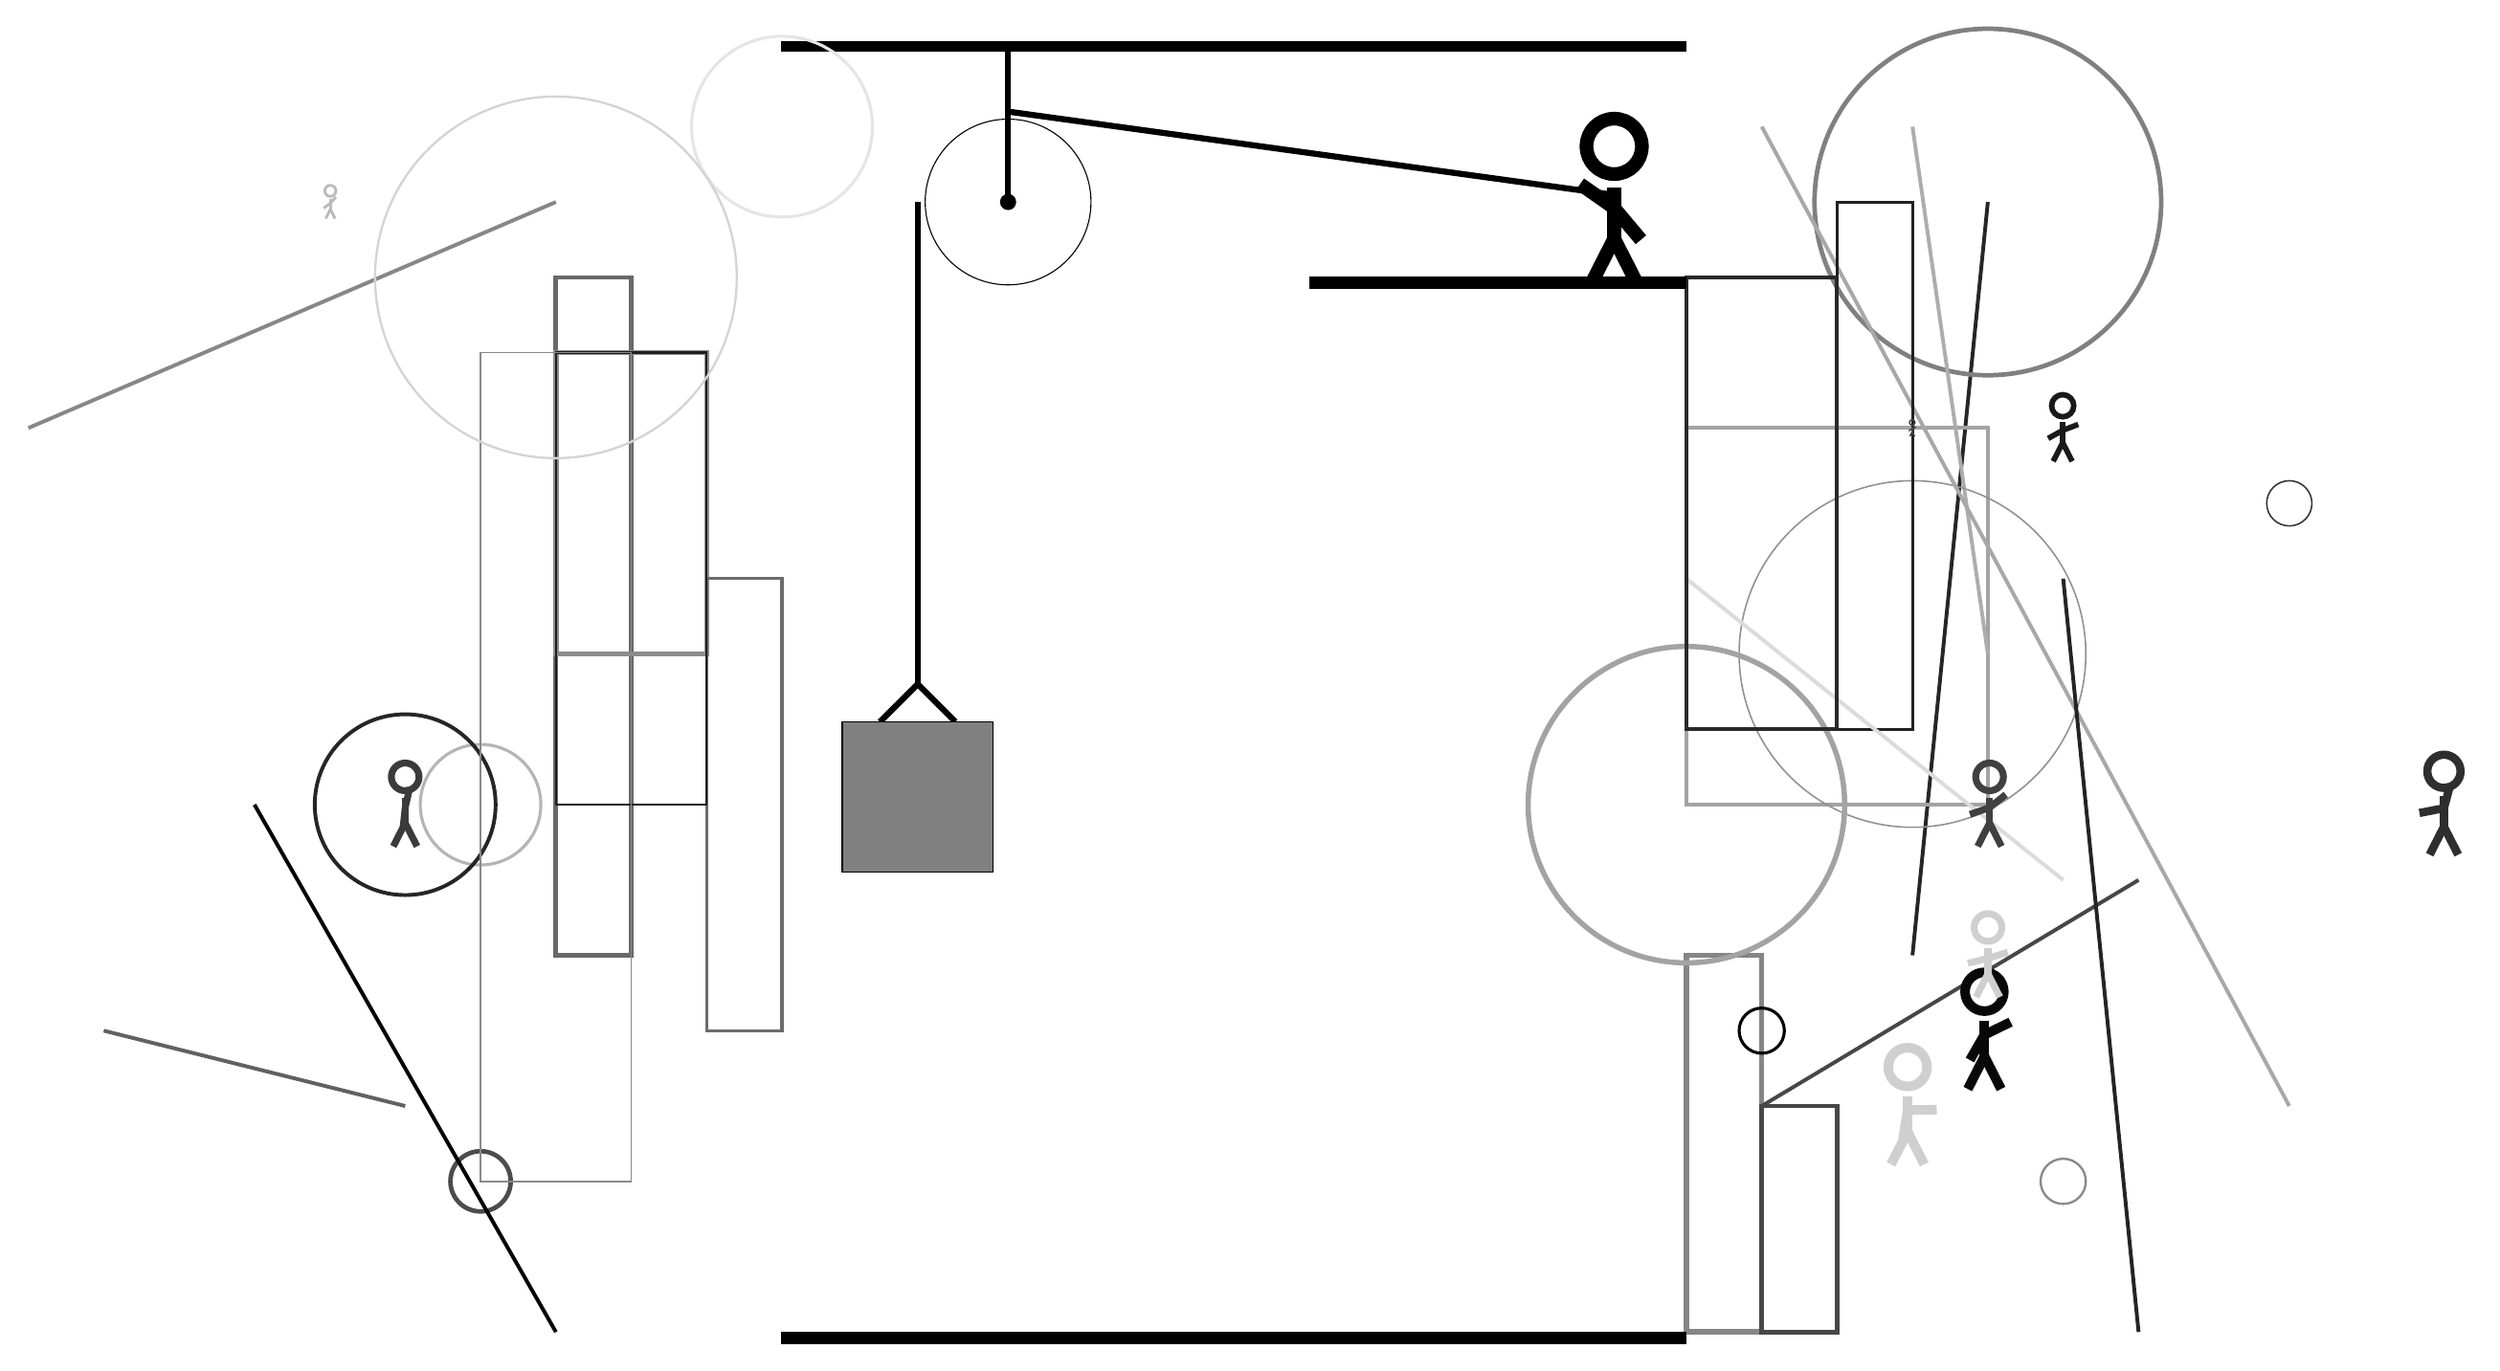
\begin{tikzpicture}
			%%%%% START %%%%%
			
			\draw[fill=black] (-2, 14) rectangle (10, 14.125);
			
			\draw (1, 12) circle (1.1);
			\draw[fill=black] (1, 12) circle (0.1);
			\draw[line width=0.8mm] (1, 14) -- (1, 12);
			
			\draw[line width=0.8mm](-0.7, 5.1) --  (-0.2, 5.6) -- (0.3, 5.1);
			\draw[fill=black!50] (-1.2, 5.1) rectangle (0.8, 3.1);
			
			\draw[line width=0.8mm](-0.2, 12) -- (-0.2, 5.6);
			\centerarc[line width=0.8mm](1, 12)(90:180:1.2000000000000002)
			\draw[line width=0.8mm](1, 13.2) -- (9, 12.1);
			
			\draw[line width=0.7mm, color=black!48] (10, 2) rectangle (11, -3);
			
			\draw[line width=0.5mm, color=black!85](13, 2) -- (14, 12);
			\draw[line width=0.6mm, color=black!59] (-4, 2) rectangle (-5, 11);
			\draw [line width=0.6mm, color=black!70](-6, -1) circle (0.4);
			\node[line width=0.5mm, color=black!19] at (13, 0) {\Strichmaxerl[7][81][1]};
			\draw[line width=0.5mm, color=black!36] (10, 4) rectangle (14, 9);
			
			\draw [line width=0.6mm, color=black!50](14, 12) circle (2.3);
			
			\draw[line width=0.5mm, color=black!100](-5, -3) -- (-9, 4);
			\draw[line width=0.5mm, color=black!72](11, 0) -- (16, 3);
			\node[line width=0.2mm, color=black!27] at (-8, 12) {\Strichmaxerl[2][37][48]};
			
			\node[line width=0.4mm, color=black!77] at (-7, 4) {\Strichmaxerl[5][84][77]};
			
			\draw[line width=0.5mm, color=black!32](14, 6) -- (13, 13);
			\draw [line width=0.2mm, color=black!43](13, 6) circle (2.3);
			\draw[line width=0.7mm, color=black!45] (-3, 10) rectangle (-5, 6);
			\draw[line width=0.5mm, color=black!34](11, 13) -- (18, 0);
			\draw[line width=0.4mm, color=black!87] (12, 12) rectangle (13, 5);
			
			\draw [line width=0.4mm, color=black!29](-6, 4) circle (0.8);
			
			\draw[line width=0.4mm, color=black!58] (-3, 7) rectangle (-2, 1);
			\node[line width=0.5mm, color=black!97] at (14, 1) {\Strichmaxerl[7][60][26]};
			\node[line width=0.4mm, color=black!74] at (13, 9) {\Strichmaxerl[1][34][21]};
			\draw[line width=0.5mm, color=black!86](15, 7) -- (16, -3);
			
			\node[line width=0.6mm, color=black!19] at (14, 2) {\Strichmaxerl[5][14][17]};
			
			\draw[line width=0.5mm, color=black!14](10, 7) -- (15, 3);
			\draw [line width=0.5mm, color=black!85](-7, 4) circle (1.2);
			\draw[line width=0.5mm, color=black!47](-5, 12) -- (-12, 9);
			
			\draw [line width=0.4mm, color=black!10](-2, 13) circle (1.2);
			
			\draw[line width=0.3mm, color=black!88] (-3, 10) rectangle (-5, 4);
			\draw [line width=0.4mm, color=black!99](11, 1) circle (0.3);
			\draw [line width=0.2mm, color=black!79](18, 8) circle (0.3);
			\draw[line width=0.5mm, color=black!62](-7, 0) -- (-11, 1);
			\draw[line width=0.2mm, color=black!46] (-4, 10) rectangle (-6, -1);
			\node[line width=0.2mm, color=black!82] at (20, 4) {\Strichmaxerl[6][11][75]};
			\draw [line width=0.3mm, color=black!17](-5, 11) circle (2.4);
			
			\draw[line width=0.6mm, color=black!72] (11, 0) rectangle (12, -3);
			\node[line width=0.3mm, color=black!75] at (14, 4) {\Strichmaxerl[5][19][39]};
			\draw [line width=0.7mm, color=black!36](10, 4) circle (2.1);
			\draw [line width=0.3mm, color=black!46](15, -1) circle (0.3);
			\node[line width=0.7mm, color=black!90] at (15, 9) {\Strichmaxerl[4][29][21]};
			\draw[line width=0.5mm, color=black!84] (10, 11) rectangle (12, 5);
			
			\node at (9, 12) {\Strichmaxerl[10][-35][-50]};
			\draw[fill=black] (5, 11) rectangle (10, 10.85);
			
			\draw[fill=black] (-2, -3) rectangle (10, -3.15);
			
			%%%%% END %%%%%
		\end{tikzpicture}
	\end{figure}	
\end{document}